\section{Feature Importance}\label{sec:feature_imp}
Because our feature vector is directly correlated with the templates of each species,
it is possible to determine their impact and quality by computing feature
importances from our classifier.
This allows us to reduce the number of templates involved in classifying a given
sample, significantly cutting down the cost of template matching per species.
Feature importances also help us analyse the preprocessing performance in detail,
as well as view inter-species correlations in cases where there is a high
level of confusion.

\subsection{In Random Forests}

The two most common methods for retrieving feature importance from a random
are detailed in this section.

\subsubsection{Mean decrease accuracy}
One method for measuring the impact of each feature is through the mean decrease
in accuracy.
With this method, the impact of removing each feature one-by-one is measured.
This method may be sensitive to the random nature of the classifier, so multiple
runs may be required to eliminate any variance.
This can be prohibitively expensive.

\subsubsection{Mean decrease impurity}
Because tree nodes in a random forest correlate directly with a specific
feature, it is possible to directly measure or estimate the importance of each
feature by determining the probability of a node in a tree being traversed over 
the number of nodes in the forest.
This is known as the mean decrease impurity, or gini importance, which is what
we use in Sckikit's random forest classifier implementation.

\subsection{Results and Analysis}\label{sec:template_analysis}
Measuring feature importances exposes 43\% (15343 out of 35773) templates as 
completely irrelevant for classification within our dataset
(Figure~\ref{fig:fimp_a}).
Removing these features shows no reduction in accuracy, and a significant speedup
during template matching is potentially gained.

There exist 35773 templates distributed across 20 spectrograms for each
of the 12 species selected.
When classifying a new sample, its spectrogram is be cross-correlated with
each of the templates.
This operation is extremely expensive, taking up to 70 hours, or approximately
5.8 hours per sample, 0.6 seconds per template on average.

The aim is therefore to reduce the feature count as much as possible while
retaining the highest possible accuracy by determining an appropriate importance
cutoff.
Removing features and reevaluating the classifier takes no significant time in
contrast to template extraction and may therefore be done by iteratively removing
and checking classifier accuracy, adjusting the importance cutoff accordingly.
This however will of course only reduce the time required to classify new samples.
We have not done this however.\\

Feature reduction is also beneficial to feature extraction, specifically when
merging the results of two batches.
Templates with importance scores equalling or close to zero can be safely removed
from the set before merging with another batch, saving a considerable amount of time.
Although we have not done this in practice the estimated amount of time saved is
in the order of 2 and a half hours per sample, assuming a consistent 43\%
template reduction rate.

\begin{figure}[!htb]
  \centering
  \begin{subfigure}[b]{1\textwidth}
    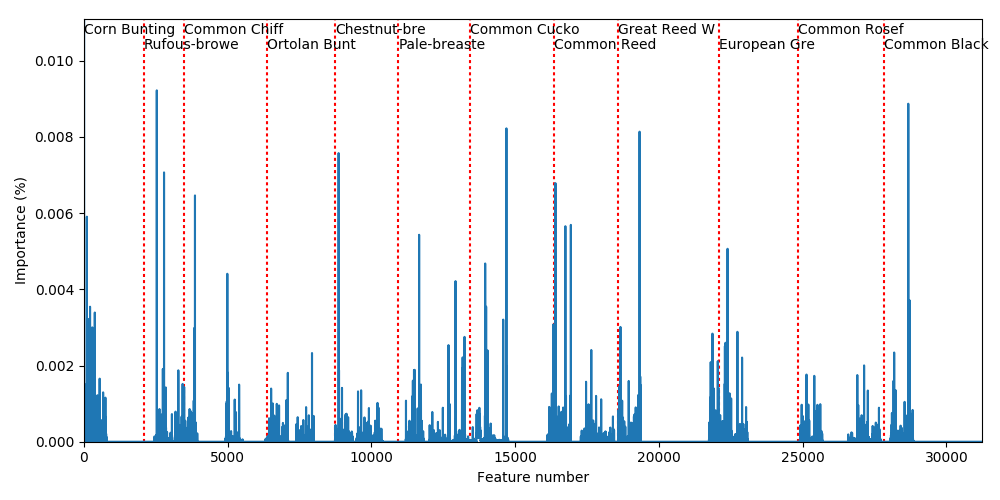
\includegraphics[width=1.0\textwidth]{imp1}
    \caption{}
    \label{fig:fimp_a}
  \end{subfigure}
  \begin{subfigure}[b]{1\textwidth}
    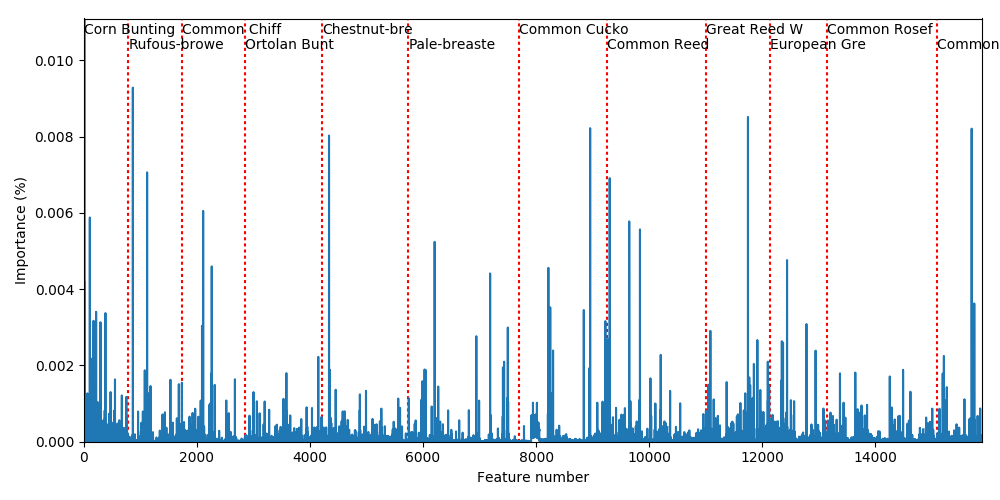
\includegraphics[width=1.0\textwidth]{imp2}
    \caption{}
    \label{fig:fimp_b}
  \end{subfigure}
  \caption{Visualisation of feature importances before (a) and after (b)
    reduction}
  \label{fig:fimp}
\end{figure}


\subsubsection{Survey}
Because we are using a single algorithm to classify the entire label set, it is
difficult to determine individual label-specific importances of each feature.
The importance figures extracted here represent the overall impact of each
template in classifying \emph{all} labels.

To gain some insight into the preferable structure of a template, we have
extracted the top ten most influential templates from the best (Acc. 99\%) and
worst performing (Acc. 75\%) label.
From this selection the Common Blackbird's templates (Figure~\ref{fig:impt2}
show slightly less
inter-correlation than those of the Ortolan Bunting (Figure~\ref{fig:impt1}).
It is somewhat surprising that some of these features, although appearing to be
overly generic, are the most influential.

It may be possible that these high importance features score well because they
fit only to very specific samples, or that they are excellent discriminators
for other species.
It is difficult to make further analysis without label-specific importances
and measuring the effect of modifying the feature vector further.

\begin{figure}[!htb]
  \centering
  \begin{subfigure}[b]{0.2\textwidth}
    \centering
    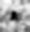
\includegraphics{XC287189-94}
  \end{subfigure}%
  \begin{subfigure}[b]{0.2\textwidth}
    \centering
    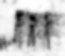
\includegraphics{XC155604-34}
  \end{subfigure}%
  \begin{subfigure}[b]{0.2\textwidth}
    \centering
    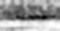
\includegraphics{XC104005-11}
  \end{subfigure}%
  \begin{subfigure}[b]{0.2\textwidth}
    \centering
    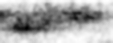
\includegraphics{XC139764-68}
  \end{subfigure}%
  \begin{subfigure}[b]{0.2\textwidth}
    \centering
    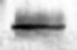
\includegraphics{XC104005-68}
  \end{subfigure}
  \begin{subfigure}[b]{0.2\textwidth}
    \centering
    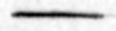
\includegraphics{XC120961-1}
  \end{subfigure}%
  \begin{subfigure}[b]{0.2\textwidth}
    \centering
    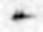
\includegraphics{XC120962-2}
  \end{subfigure}%
  \begin{subfigure}[b]{0.2\textwidth}
    \centering
    
\includegraphics{XC243644-11}
  \end{subfigure}%
  \begin{subfigure}[b]{0.2\textwidth}
    \centering
    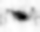
\includegraphics{XC155604-31}
  \end{subfigure}%
  \begin{subfigure}[b]{0.2\textwidth}
    \centering
    
\includegraphics{XC253633-72}
  \end{subfigure}%
  \caption{Top 5 most influential features from the Ortolan Bunting}
  \label{fig:impt1}
\end{figure}

\begin{figure}[!htb]
  \centering
  \begin{subfigure}[b]{0.2\textwidth}
    \centering
    
\includegraphics{XC312276-7}
  \end{subfigure}%
  \begin{subfigure}[b]{0.2\textwidth}
    \centering
    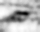
\includegraphics{XC312276-340}
  \end{subfigure}%
  \begin{subfigure}[b]{0.2\textwidth}
    \centering
    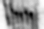
\includegraphics{XC312276-204}
  \end{subfigure}%
  \begin{subfigure}[b]{0.2\textwidth}
    \centering
    
\includegraphics{XC30284-109}
  \end{subfigure}%
  \begin{subfigure}[b]{0.2\textwidth}
    \centering
    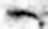
\includegraphics{XC238539-67}
  \end{subfigure}
  \begin{subfigure}[b]{0.2\textwidth}
    \centering
    
\includegraphics{XC30284-117}
  \end{subfigure}%
  \begin{subfigure}[b]{0.2\textwidth}
    \centering
    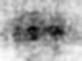
\includegraphics{XC30284-154}
  \end{subfigure}%
  \begin{subfigure}[b]{0.2\textwidth}
    \centering
    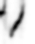
\includegraphics{XC312276-27}
  \end{subfigure}%
  \begin{subfigure}[b]{0.2\textwidth}
    \centering
    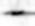
\includegraphics{XC312276-252}
  \end{subfigure}%
  \begin{subfigure}[b]{0.2\textwidth}
    \centering
    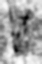
\includegraphics{XC238539-231}
  \end{subfigure}
  \caption{Top 5 most influential features from the Common Blackbird}
  \label{fig:impt2}
\end{figure}
